\documentclass[paperwidth=100cm,paperheight=120cm]{baposter}
%\documentclass[a0,portrait,final]{baposter_old}
%\documentclass[a4shrink,portrait,final]{baposter}
%\documentclass[a0,landscape,final]{baposter}

%\documentclass[a4shrink,portrait,final]{baposter}
% Usa a4shrink for an a4 sized paper.

\usepackage[utf8]{inputenc}

\tracingstats=2
\usepackage{verbatim}
%\usepackage{lipsum}
\usepackage{graphicx}

\usepackage{times}
\usepackage{calc}
\usepackage{amsmath}
\usepackage{amssymb}
\usepackage{relsize}
%\usepackage{multirow}
\usepackage{bm}
\usepackage{multicol}
\usepackage{pgfbaselayers}
\pgfdeclarelayer{background}
\pgfdeclarelayer{foreground}
\pgfsetlayers{background,main,foreground}
\usepackage{helvet}
%\usepackage{bookman}
\usepackage{palatino}
\newcommand{\captionfont}{\footnotesize}
\selectcolormodel{cmyk}
\graphicspath{{images/}}

\newcommand{\DT}{\Delta T}
% Some math symbols used in the text
\newcommand{\Matrix}[1]{\begin{bmatrix} #1 \end{bmatrix}}
\newcommand{\Vector}[1]{\Matrix{#1}}
\newcommand*{\SET}[1]  {\ensuremath{\mathcal{#1}}}
\newcommand*{\MAT}[1]  {\ensuremath{\mathbf{#1}}}
\newcommand*{\VEC}[1]  {\ensuremath{\bm{#1}}}
\newcommand*{\CONST}[1]{\ensuremath{\mathit{#1}}}
\newcommand*{\norm}[1]{\mathopen\| #1 \mathclose\|}% use instead of $\|x\|$
\newcommand*{\abs}[1]{\mathopen| #1 \mathclose|}% use instead of $\|x\|$
\newcommand*{\absLR}[1]{\left| #1 \right|}% use instead of $\|x\|$
\def\norm#1{\mathopen\| #1 \mathclose\|}% use instead of $\|x\|$
\newcommand{\normLR}[1]{\left\| #1 \right\|}% use instead of $\|x\|$

%Author's defs
\def\afi#1{$^{(#1)}$}
\def\bu{\textcolor{red}{\textbullet~}}
%---------- Author's commands---------------------------------
%\def\rsun{R$_{\rm SUN}$}
\def\bA{{\bf A}}
\def\ba{{\boldsymbol{a}}}
\def\bB{{\bf B}}
\def\bb{{\bf b}}
\def\bC{{\bf C}}
\newcommand{\dd}{\mathrm{d}}
\def\bD{{\bf D}}
\def\bd{{\bf d}}
\def\be{{\boldsymbol{e}}}
\def\bF{{\bf F}}
\def\bff{{\bf f}}
\def\bg{{\bf g}}
\def\bG{{\bf G}}
\def\bh{{\bf h}}
\def\bH{{\bf H}}
\def\bi{{\bf i}}
\def\bI{{\boldsymbol{I}}}
\def\bk{{\bf k}}
\def\bK{{\bf K}}
\def\bM{{\bf M}}
\def\bn{{\boldsymbol{n}}}
\def\boo{{\boldsymbol{o}}}
\def\bp{{\boldsymbol{p}}}
\def\bP{{\bf $P$}}
\def\bq{{\boldsymbol{q}}}
\def\bQ{{\bf Q}}
\def\br{{\boldsymbol{r}}}
\def\bR{{\bf R}}
\def\bs{{\bf s}}
\def\bS{{\bf S}}
\def\bt{{\bf t}}
\def\bT{{\bf T}}
\def\bU{{\bf U}}
\def\bW{{\bf W}}
\def\bx{{\bf x}}
\def\by{{\bf y}}
\def\bSigma{{\bf \Sigma}}
\def\bLambda{{\bf \Lambda}}
\def\blambda{{\bf \lambda}}
\def\bN{{\bf \mathcal{N}}}
\def\bchi{\boldsymbol{\chi}}
\def\bxi{\boldsymbol{\xi}}
\def\bzeta{\boldsymbol{ \zeta}}
\newcommand{\lbl}{\mbox{\boldmath $\hat{l}$}}
\newcommand{\lpl}{\mbox{\boldmath $\hat{p}$}}
\def\deg{$^\circ$}
\def\mdeg{^\circ}
\def\bbp{{\bf p}}

\def\rsun{R$_\odot$}
\def\deg{$^\circ$}
\def\mdeg{^\circ}
%\def\tr{\textcolor{blue}{$\blacktriangleright$~}}
\def\bu{\textcolor{red}{\textbullet~}}
\def\tr{\bu}
\def\bbu{\textbullet~}
\def\cmsq{cm$^2$}
\def\cmcu{cm$^3$}
\def\azul#1{\textcolor{blue}{#1}}
\def\eazul#1{\textcolor{blue}{\emph{#1}}}
\def\rojo#1{\textcolor{red}{#1}}

\def\verde#1{\textcolor{green}{#1}}
\def\orange#1{\textcolor{orange}{#1}}
\def\bL{{\bf L}}

\def\bazul#1{\textcolor{blue}{\bf\tt #1}}
\def\brojo#1{\textcolor{red}{\bf\tt #1}}

\def\ldem{{\sf LDEM}}


%----------------------------------------------------------------------

% Multicol Settings
\setlength{\columnsep}{0.2em}
\setlength{\columnseprule}{0mm}

% Save space in lists. Use this after the opening of the list
\newcommand{\compresslist}{%
\setlength{\itemsep}{1pt}%
\setlength{\parskip}{0pt}%
\setlength{\parsep}{0pt}%
}

% Begin of Document
\begin{document}

% Here starts the poster
% Format it to your taste with the options
% Define some colors
\definecolor{silver}{cmyk}{0,0,0,0.3}
\definecolor{yellow}{cmyk}{0,0,0.9,0.0}
\definecolor{reddishyellow}{cmyk}{0,0.22,1.0,0.0}
\definecolor{black}{cmyk}{0,0,0.0,1.0}
\definecolor{darkYellow}{cmyk}{0,0,1.0,0.5}
\definecolor{darkSilver}{cmyk}{0,0,0,0.1}
\definecolor{lightyellow}{cmyk}{0,0,0.3,0.0}
\definecolor{lighteryellow}{cmyk}{0,0,0.1,0.0}
\definecolor{lighteryellow}{cmyk}{0,0,0.1,0.0}
%\definecolor{lightestyellow}{cmyk}{0,0,0.05,0.0}
\definecolor{MyLightMagenta}{cmyk}{0.1,0.8,0,0.1}
%\definecolor{MyDarkBlue}{rgb}{0.1,0,0.55} 
%\definecolor{MyLightBlue}{rgb}{0.1,0,0.1} 
\definecolor{MyDarkBlue}{cmyk}{1,0.7,0.4,0}
\definecolor{MyLightBlue}{cmyk}{0.4,0.2,0.2,0}
%\definecolor{MyDarkBlue}{cmyk}{1,0.5,0.5,0}
\definecolor{MyLightBlue}{cmyk}{0.13,0.08,0,0}
\definecolor{MyLightBlue}{cmyk}{0.2,0.13,.13,0}
\definecolor{MyLightBlue}{cmyk}{0.3,0.2,.2,0}
\definecolor{MyLightBlue}{cmyk}{0.15,0.1,.1,0}
\definecolor{light-gray}{gray}{0.85}
\definecolor{light-gray2}{gray}{0.85}
%%

\typeout{Poster Starts}

\background{
  \begin{tikzpicture}[remember picture,overlay]
    \draw (current page.north west)+(0,2em) node[anchor=north west]{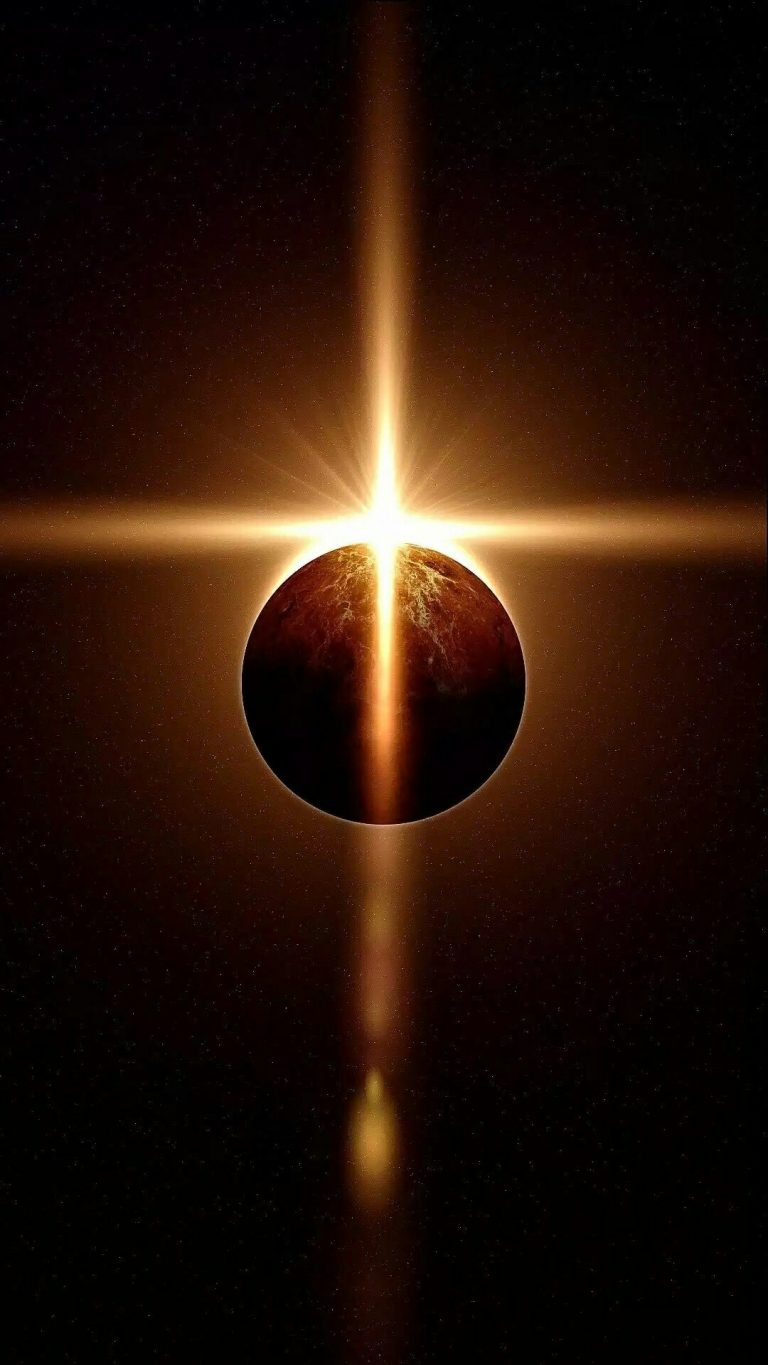
\includegraphics[width=\paperwidth]{solar-eclipse-wallpaper-iphone-768x1365.jpg}};%{aconcagua.jpg}};%fondo1.jpg
    %[remember picture,overlay]\node[opacity=0.5] at (current page.center){\includegraphics[width=\paperwidth,height=\paperheight]{plasma2.png}};
  \end{tikzpicture}%
}

\newlength{\leftimgwidth}
\begin{poster}%
  % Poster Options
  {
  % Show grid to help with alignment
  %grid=no,
  grid=false,
  % Column spacing
  colspacing=1em,
  % Color style
  bgColorOne=MyLightBlue,%lighteryellow,
  bgColorTwo=MyLightBlue,%lightestyellow,
  borderColor=MyDarkBlue,%reddishyellow,
  headerColorOne=MyDarkBlue,
  headerColorTwo=white,%reddishyellow,
  headerFontColor=white,
  boxColorOne=white,%MyLightBlue,
  boxColorTwo=white,%MyLightBlue,
  % Format of textbox
  textborder=roundedleft,
  % Format of text header
  %eyecatcher=yes,
   eyecatcher=true,
  headerborder=open,
  headerheight=0.09\textheight,
  headershape=roundedright,
  headershade=plain,
  headerfont=\large\sf, %Sans Serif
 %boxshade=shadetb,
 boxshade=shadelr,
  %boxshade=none,%shade-lr,
%background=shade-tb,
  %background=plain,
  background=user,
  linewidth=2pt,
  columns=4
  }
  {\setlength\fboxsep{0pt}\setlength\fboxrule{0.5pt}
  \fbox{
\includegraphics[height=6.em]{logo_IAFE.jpg}}}
 % Title
 {\sf\textcolor{light-gray}%{MyDarkBlue}
 {\vskip -0.2cm \bf \LARGE Thermodynamics of the Inner Solar Corona: \\
  A Tomographic Validation Study of the AWSoM Model}}
% Authors
{ \footnotesize\sf
{\bf \footnotesize
\textcolor{light-gray2}{Diego G. Lloveras\afi{1}}\textcolor{MyDarkBlue}{(dlloveras@iafe.uba.ar)},
\textcolor{light-gray2}{C. Mac Cormack\afi{1}, A.M. Vásquez\afi{1}, N. Sachdeva\afi{2}, W. Manchester IV\afi{2}, B. Van der Holst\afi{2}, R.A. Frazin\afi{2}}}\\
%\vskip 0.05cm
\textcolor{light-gray2}{\afi{1}Instituto de Astronom\'\i a y F\'\i sica del Espacio (CONICET-UBA), CC
67 - Suc 28, Ciudad de Buenos Aires, Argentina.\\
%\vskip 0.05cm
{\afi{2}Department of Climate and Space Sciences and Engineering (CLaSP, University of Michigan).}
\vskip -0.5cm
}
}
% University logo
{\setlength\fboxsep{0pt}\setlength\fboxrule{0.5pt}
  \fbox{
\includegraphics[height=6.em]{logo_CLASP.pdf}}}

% Now define the boxes that make up the poster
%%%---------------------------------------------------------------------------
%%% Each box has a name and can be placed absolutely or relatively.
%%% The only inconvenience is that you can only specify a relative position 
%%% towards an already declared box. So if you have a box attached to the 
%%% bottom, one to the top and a third one which should be in between, you 
%%% have to specify the top and bottom boxes before you specify the middle 
%%% box.

\headerbox{{Abstract}}{name=resumen,column=0,row=0,span=4}{
\begin{center} 
{\sf To advance the understanding of the physics of the solar corona, magnetohydrodynamic (MHD) three-dimensional (3D) models need to be validated with observations. To that end, differential emission measure tomography (DEMT) provides global 3D maps of the electron density and temperature in the inner corona (1.0-1.25 Rsun). In combination with models of the coronal magnetic field, it allows estimating the energy input flux required at the coronal base to maintain thermodynamically stable coronal structures. Hence, the DEMT analysis can be useful to tune up the model's Alfven wave amplitudes and dissipation rates. Here, a DEMT validation study of the latest version of the  Alfvén Wave Solar Model (AWSoM) of the Space Weather Modeling Framework (SWMF) is reported. The analysis is carried out for Carrington rotations selected from the previous solar minimum and the current declining phase of solar cycle 24. The capability of the model to reproduce the tomographic products is discussed, and the need for improvements in the model is evaluated.}
\end{center}
}

\headerbox{DEMT Technique}{name=demt2,column=0,below=resumen,span=2}{
{\footnotesize\sf
DEMT technique calculates the Local Differential Emission Measure (LDEM) in each 3D volume element from series of EUV images taken during a solar rotation. By computing LDEM moments, 3D distributions of electronic density and temperature can be obtained. In this work DEMT was applied to EUV (Extreme Ultraviolet) images taken by the Extreme Ultraviolet Imager (EUVI) instrument on board the STEREO-B spacecraft during Carrington Rotation (CR)-2082 and by Atmospheric Imaging Assembly (AIA) instrument on board SDO during CR-2208.

}
}
\headerbox{Alfvén Wave Solar Model (AWSoM)}{name=awsom,column=2,below=resumen,span=2}{
{\footnotesize\sf
AWSoM is a global 3D MHD model of the solar chromosphere and corona driven by magnetogram data (van Der Holst et al., 2014). At the coronal base, Alfvén waves are reflected and generate a turbulent cascade. The dissipation of this cascade contributes to the coronal heating. Taking into account the turbulence generated by low frequency Alfvén waves, the model solves MHD equations and obtains 3D distributions of electronic density and temperature, together with many other physical quantities. In this work we perform a steady-state simulation of CR-2082 and CR-2208 using synoptic magnetograms from the Michelson Doppler Imager (MDI) instrument on board the SoHO spacecraft. 

}
}

\headerbox{Reconstrucción 3D de ${\rm N_e}$}
{name=maps2,column=0,below=demt2,span=2}{
%\azul{ \hskip 2.4cm CR-1915 \hskip 3.0cm CR-2081 \hskip 3.1cm CR-2192 }
\begin{center}
%\azul{\hskip 1cm Mínimo 1996 \hfill Mínimo 2009 \hskip 1cm}
%\vskip 0.01cm
%{\includegraphics[width=0.49\textwidth]{DEMT_ne_cr2081_run5_disk_1035Rsunmapoc_2.pdf}}
%{\includegraphics[width=0.49\textwidth]{DEMT_ne_cr2081_run5_disk_1105Rsunmapoc_2.pdf}}
%{\includegraphics[width=0.49\textwidth]{AWSoM_ne_cr2081_run5_disk_1035Rsunmapoc_2.pdf}}
%{\includegraphics[width=0.49\textwidth]{AWSoM_ne_cr2081_run5_disk_1105Rsunmapoc_2.pdf}}\\

%{\includegraphics[width=0.49\textwidth]{test_triplecaca3_Bbase_cerrado_est.pdf}}\\
\end{center}
\vskip -0.16cm
{\footnotesize\sf
Carrington maps of the electronic density at $1.035 \, {\rm R}_\odot$ (left panels) and $1.105 \, {\rm R}_\odot$ (right panels) obtained with the DEMT technique (top) and AWSoM model (bottom). Black curves denote the magnetically open/closed boundary of the AWSoM model. 

}
}

\headerbox{3D Reconstruction of ${\rm T_{e}}$}
{name=maps3,column=2,below=awsom,span=2}{
{\footnotesize\sf
%\azul{ \hskip 2.4cm CR-1915 \hskip 3.0cm CR-2081 \hskip 3.1cm CR-2192 }
%\vskip 0.01cm
\begin{center}
%\azul{\hskip 1cm Mínimo 1996 \hfill Mínimo 2009 \hskip 1cm}
%\vskip 0.01cm
%{\includegraphics[width=0.49\textwidth]{DEMT_te_cr2081_run5_disk_1035Rsunmapoc_2.pdf}}
%{\includegraphics[width=0.49\textwidth]{DEMT_te_cr2081_run5_disk_1105Rsunmapoc_2.pdf}}
%{\includegraphics[width=0.49\textwidth]{AWSoM_te_cr2081_run5_disk_1035Rsunmapoc_2.pdf}}
%{\includegraphics[width=0.49\textwidth]{AWSoM_te_cr2081_run5_disk_1105Rsunmapoc_2.pdf}}\\
\end{center}
}
}

\headerbox{Global Comparison as a Function of Height}
{name=alturas,column=0,below=maps2,span=2}{
{\footnotesize\sf
For each physical quantity $X$, we measure its relative difference between the AWSoM and DEMT results at each coronal computational cell $i$ as: 
$Q_i\,\equiv\,2\,\frac{|X_{\rm AWSoM} - X_{\rm DEMT}|}{(X_{\rm AWSoM} + X_{\rm DEMT})}$.
\begin{center}
%\azul{\hskip 1cm Mínimo 1996 \hfill Mínimo 2009 \hskip 1cm}
%\vskip 0.01cm
%{\includegraphics[width=0.45\textwidth]{Median_Ne_full_height_run5_disk.pdf}}
%{\includegraphics[width=0.45\textwidth]{Median_Te_full_height_run5_disk.pdf}}\\
\end{center}
\vskip -0.16cm
Median value of ${\rm Q_i}$ at every height for ${\rm N_e}$ and ${\rm T_e}$ within the Streamer and each polar Coronal Hole.

}
}

\headerbox{Average Fitts to ${\rm N_e}$ and ${\rm T_{e}}$ along loops}
{name=ajuste1,column=2,below=maps3,span=2}{
{\footnotesize\sf
The DEMT and AWSoM results are then traced along each magnetic field line obtained with AWSoM model allowing a detailed thermodynamic comparison along the magnetic field. Using a hydrostatic fit for density and a linear fit for the temperature, the coronal basal density ${\rm N_{e basal}}$ (density at $1.025 \, {\rm R}_\odot$) and the mean electronic temperature ${\langle \rm T_e \rangle}$ are determined for each field line.
\begin{center}
%\azul{\hskip 1cm Mínimo 1996 \hfill Mínimo 2009 \hskip 1cm}
%\vskip 0.01cm
%{\includegraphics[width=0.49\textwidth]{ajuste_promedio_ne_lowlat_colage_testeo.pdf}}
%{\includegraphics[width=0.49\textwidth]{ajuste_promedio_ne_chs_colage_testeo.pdf}}\\
%{\includegraphics[width=0.49\textwidth]{ajuste_promedio_te_lowlat_colage_testeo.pdf}}
%{\includegraphics[width=0.49\textwidth]{ajuste_promedio_te_chs_colage_testeo_3.pdf}}\\
\end{center}
DEMT fits in solid blue lines. The dashed blue lines indicate the uncertainty (Lloveras {\rm et al.} 2017). In red lines AWSoM fits below $1.05 \, {\rm R}_\odot$ and above $1.05 \, {\rm R}_\odot$.

}
}

\headerbox{Statistical Comparison}
{name=histo,column=0,below=alturas,span=2}{
{\footnotesize\sf
\begin{center}
%\azul{\hskip 1cm Mínimo 1996 \hfill Mínimo 2009 \hskip 1cm}
%\vskip 0.01cm
%{\includegraphics[width=0.4\textwidth]{histoplot2_fullne_lowlat_colage.pdf}}
%{\includegraphics[width=0.4\textwidth]{histoplot2_fullne_chs_colage.pdf}}\\
%{\includegraphics[width=0.4\textwidth]{histoplot2_fulltm_lowlat_colage.pdf}}
%{\includegraphics[width=0.4\textwidth]{histoplot2_fulltm_chs_colage.pdf}}\\
\end{center}
\vskip -0.16cm
Frequency histograms of ${\rm N_{e basal}}$ and ${\rm \langle T_e \rangle}$ (above $1.05 \, {\rm R}_\odot$) for the Streamer and the polar Coronal Holes.

}
}

\headerbox{Conclusions}
{name=conclusions,column=2,below=ajuste1,span=2}{
{\footnotesize\sf
\bu Below $r \sim 1.05 {\rm R_{SUN}}$, the electron temperatures of AWSoM are a factor $\sim 2$ smaller than those observed with DEMT, while the electron densities are a factor $\sim 2-5$ larger.

\bu Above $\sim 1.05 {\rm R_{SUN}}$ (in both Streamers and CHs): $T_e$ agreement within $\sim 15 \%$, which is the uncertainty level of DEMT due to systematic sources. $N_e$ agreement within a factor of 2 (with AWSoM under-estimating in Streamers, and over-estimating in CHs), well beyond uncertainty.

\bu The structure of the streamer is dominated by down loops which are not modeled by AWSoM.

\bu The lack of agreement in density, as well as the evident change of behavior of the AWSoM results below/above 1.05 $R_{\rm SUN}$, are related to its treatment of the Chromosphere/Corona transition. The model is currently being udated to improve its performance. Future efforts will involve DEMT validation of its updated results.

}
}

\end{poster}%
\end{document}
